% theKATRINexperiment.tex
%

    \chapter{The KATRIN experiment}
    \label{ch:The KATRIN experiment}
    The KATRIN experiment is on its way to measure the neutrino mass or set new upper limits at precisions never achieved before. It will reach a sensitivity of \SI{500}{\milli\electronvolt}/\SI{}{\square c} excelling the previously best experiments of Mainz and Troisk by a factor of \todo{how much?}. Major challenges of the project are the requirement of ultra high vacuum, the exat knowledge of all magnetic and electic fields as well as external influences on those, the required high luminosity of the Tritium source and the reduction of background sources.
      \section{Measurement principle}
      \label{ch:The KATRIN experiment:sec:Measurement Principle}
      A generally easy principle is used to find information on the neutrino mass: The energy of electrons from tritium decay is measured with high precision and compared to the standard model's presumption for a massless neutrino: 
      \begin{equation}
      	\ce{^3_1T -> ^3_1H^+ + e^- + \bar{\nu}_e}
      \end{equation}
      As the decay's energy is distributed between the constant neutrino's rest mass and its and the elctron's kinectic energies respectively, the decay electrons will show a continous spectrum. The difference between the electron energy calculated by standard model presumptions to the extrapolated maximum electron energy from the spectrum then equals the neutrino rest mass as shown on figure \ref{fig:katrinExperiment:tritiumSpectrum}
      \begin{figure}
	\centering
      	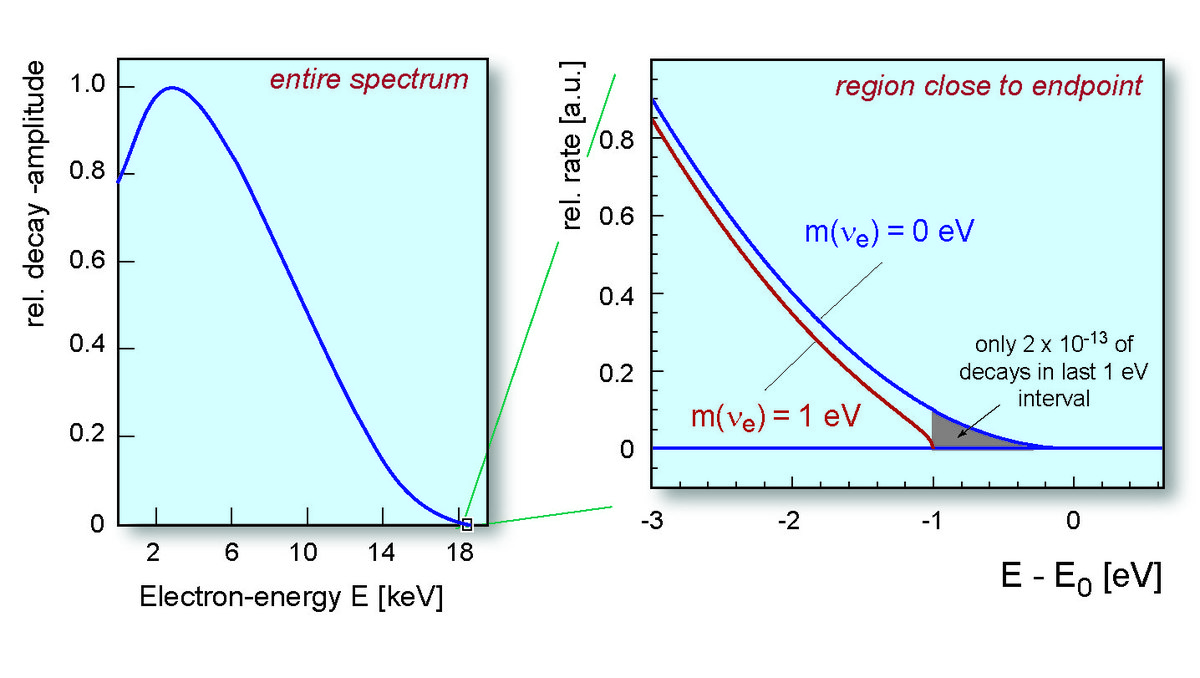
\includegraphics[width = 0.9 \textwidth]{graphics/katrinExperiment/electronSpectrum.jpg}
      	\caption{Schematic energy spectrum for electrons from tritium beta decay. On the left, the entire spectrum with the peak at the energy most emitted - around \SI{5}{\electronvolt} - can be seen. On the right, a zoom-in on the endpoint showing both the calculations for a massless and a \SI{1}{\electronvolt} neutrino. As described in the graph, rates in this region are extremely low and extrapolation through advanced software tools needs to be applied.}
      	\label{fig:katrinExperiment:tritiumSpectrum}
      \end{figure}
      A different light is shed on the simplicity of the task when considering the needed accuracy of 
      \subsection{MAC-E Filter}
      \label{ch:The KATRIN experiment:sec:MAC-E}
      A high luminousity is a major requirement for good statistics at the KATRIN experiment. This makes it impossible to use some kind of aperture to filter for electrons from Tritium decay with one momentum direction as they are emitted uniformly from the source volume and the largest amount of electrons would never reach the main spectrometer. That is why another strategy is used at KATRIN: The MAC-E filter - magnetic adiabatic collimation with electrostatic filter - which utilises the fact that, under small enough magnetic field changes, the magnetic momentum of a particle is constant; the particle can be considered adiabatic. The solenoid and coil system surrounding the main spectrometer are set up to create a strong, but smooth magnetic field gradient of several orders of magnitude. At entrance and exit of the vessel, solenoids generating fields of up to \SI{}{\tesla} are installed while in the central, widest part, the field strength reduces by a factor of \todo{factors and field strengths}. This area is called the analysing plane. According to
      \begin{equation}
      	\mu = \frac{E_{\bot}}{B} = const
      \end{equation}
      the momentum will align with the magnetic field lines as the field weakens. In the edge case of $B\rightarrow 0$ in the analysing plane, the momentum would need to be exactly parallel to the field as the transversal motion needs to approach 0 as well so that $E_\bot\rightarrow 0$. In the case of 

       This allow for an angular acceptance of 2$\pi$.
      \section{Experimental setup}
      \label{ch:The KATRIN experiment:sec:Experimental setup}
      The KATRIN experiment is made up of different section all fulfilling their own important purpose in the whole setup. We start off with the production of tritium electrons in the very south. These are guided magnetically northwards through pumping tracks removing hydrogen ions and other residual gases in the process on through the two spectrometers posing as a energetic high pass filter to the focal plane detector registering them. It follows a more detailed description of the single components.
      
      \subsection{Source Side and Transport Section}
      \label{ch:The KATRIN experiment:sec:Experimental setup:subsec:sourceSide}
      The required high luminousity is achieved by using a gaseous Tritium source. In a solid, most electrons from decays inside the structure would be resorbed quickly and be unavailable for analysis. The gase's large advantage is that not only the surface facing the detector emits electrons at the desired spectrum, but the whole volume covered by the magnetic flux tube arriving at the detector can be utilised. Of course, new challenges arise from the decision to use gas instead of solids: The spectrometers further down the system require for ultra high vacuum, for the main spectrometer in the order of \SI{e-11}{\milli\bar}. As the Tritium pressure is in the order of \SI{10e-3}{\milli\bar} and the source needs to be windowless - as no electron transparent window is known to stand such pressure differences - the pressure must be reduced to desired values without any physical barrier. 
      For that purpose, after being allowed to decay inside the WGTS, the windowless gaseous tritium source, electrons fly on through DPS and CPS, the differential- and cryogenic pumping sections. In the former, pressure is actively reduced by the use of turbo pumps. Afterwards, the CPS uses strongly cooled walls to freeze residual gas, always keeping the information carrying electrons away from those by magnetic guidance.
      \subsection{Pre-Spectrometer}
      \label{ch:The KATRIN experiment:sec:Experimental setup:subsec:PreSpectrometer}
      The pre-spectrometer was built in Munster and works on the same principle as the main spectrometer, although being a lot smaller. It is installed to reduce the flux to the main spectrometer, and by that the possible amount of stored electrons inside the main vessel. The pre-spectrometer has a single layer of wires as a inner electrode to shield against externally induced electrons. It is made to 
      \subsection{Main Spectrometer}
      \label{ch:The KATRIN experiment:sec:Experimental setup:subsec:MainSpec}
      The largest component of all is the main spectrometer. With a diameter of \SI{9}{\meter} and a length of over \SI{24}{\meter}, it incorporates around \SI{1400}{\cubic\meter} that need to be evacuated to extremely high vacuum of < \SI{e-11}{\milli\bar}. The vessel is equipped with two layers of electrodes on a comb-like structure. This setup reduces the number of secondary electrons from the spectrometer walls entering the flux tube's volume. Keeping that count low, the rate of those electrons not reflected magnetically due to imperfect symmetries is reduced to the sub-\SI{}{\electronvolt} level. The layer made from thinner wires further to the inside shields the spectrometer volume from the one further towards the wall as cosmic rays may unleash elecrons there as well. 
      
      \subsection{Focal Plane Detector System}
      \label{ch:The KATRIN experiment:sec:Experimental setup:subsec:FPD system}
      The main detector is located at the very north of the experiment. It is made up of a silicon wafer divided into 148 pixels accessed by pin connectors. The pattern is dartboard-like, multiple pixels with the same distance to the center form rings. Every pixel has the same surface area, making rates more easily comparable - that is if the magnetic flux through the areas is as homogenous as in this experiment.
      \subsection{Solenoids, LFCS and EMCS system}
      To achieve magnetic guidance in the way explained above, a sophisticated system of supraconduting solenoids, the low field correction system LFCS and the earth magnetic field compensation system EMCS have been installed \cite{airCoilSystem}. These make sure that the path of flight is kept away from the wall and can be considered adiabatic, that penning traps are avoided as far as possible, that the earth magnetic field is compensated for and, most importantly, that the field drop to the analysis plane is of the order of \todo{order?} so the spectrometers resolution will achieve desired values.
      \label{ch:The KATRIN experiment:sec:Experimental setup:subsec:Solenoids, LFCS and EMCS system}
      

      \subsection{Background sources}
      \label{ch:The KATRIN experiment:sec:Experimental setup:subsec:BackgroundSources}
      Different sources contribute to the background of electrons arriving at the detector that are not from tritium decay. First, there is background due to stored electrons. Penning traps cause electrons with fitting energies to be trapped in a potential cup. Discharges of those traps due to 